\chapter{Author Extraction Example}\label{app:cha-author-extraction-example}
\section{Factor Product}\label{app:sec-factor-product}
\begin{table}[H]
\centering
$\Psi(LN_1,FN_2,EC_2)$\par
\smallskip
\begin{tabular}{c c c l}
 \toprule
 $LN_1$ & $FN_2$ & $EC_2$ & \multicolumn{1}{c}{Value} \\
 \midrule
 $false$ & $false$ & $false$ & $(10\cdot10)\cdot30=3000$\\
 $false$ & $false$ & $true$  & $(20\cdot20)\cdot30=12000$\\
 $false$ & $true$  & $false$ & $(10\cdot10)\cdot1\ \ =100$\\
 $false$ & $true$  & $true$  & $(20\cdot1\ \ )\cdot1\ \ =20$\\
 $true$  & $false$ & $false$ & $(10\cdot10)\cdot1\ \ =100$\\
 $true$  & $false$ & $true$  & $(1\ \ \cdot20)\cdot1\ \ =20$\\
 $true$  & $true$  & $false$ & $(10\cdot10)\cdot10=1000$\\
 $true$  & $true$  & $true$  & $(1\ \ \cdot\ \ 1)\cdot10=10$\\
 \bottomrule
\end{tabular}
\caption{Results of the \gls{factor product} $(\Psi(LN_1,EC_2)\times\Psi(FN_2,EC_2))\times\Psi(LN_1,FN_2)$ of the \glspl{factor} in \Cref{tab:example-factors}. For an exemplary calculation see \Cref{app:subsec-gd-example-calculation}.}
\label{tab:example-factor-product}
\end{table}
\section{Gibbs Distribution}\label{app:sec-gibbs-distribution}
\subsection{Exemplary Calculation}\label{app:subsec-gd-example-calculation}
The following calculation is based on \gls{factor graph} (a) in \Cref{fig:example-factor-graphs} with $\mathcal{X}=\{LN_1,FN_2,EC_2\}$.
It uses the \glspl{factor} defined in \Cref{tab:example-factors}.
\begin{subequations}
\begin{equation*}
\begin{split}
  \tilde{P}(LN_1{=}true,FN_2{=}true,EC_2{=}false)&=\prod_{k=1}^{K}\Psi_k\left(\mathbf{D}_k\right) \\
  &=(\Psi(LN_1{=}true,EC_2{=}false)\\
  & \hspace{2em}\times\Psi(FN_2{=}true,EC_2{=}false))\\
  & \hspace{2em}\times\Psi(LN_1{=}true,FN_2{=}true)\\
  &=(10\cdot10)\cdot10\\
  &=1000\\[1em]
\end{split}
\end{equation*}
\begin{equation*}
\begin{split}
  Z&=\sum_{EC_2,FN_2,LN_1}\tilde{P}\left(LN_1,FN_2,EC_2\right)\\
  &=\Psi(LN_1{=}false,FN_2{=}false,EC_2{=}false)\\
  &\hspace{2em}+\Psi(LN_1{=}false,FN_2{=}false,EC_2{=}true)\\
  &\hspace{2em}+\dots\\
  &\hspace{2em}+\Psi(LN_1{=}true,FN_2{=}true,EC_2{=}true)\\
  &= 16250\\[1em]
\end{split}
\end{equation*}
\begin{equation*}
\begin{split}
  P(LN_1{=}true,FN_2{=}true,EC_2{=}false)&=\frac{1}{Z}\tilde{P}\left(LN_1{=}true,FN_2{=}true,EC_2{=}false\right) \\
  &=\frac{1}{16250}\cdot1000\\
  &\approx0.0615\\
\end{split}
\end{equation*}
\end{subequations}
\subsection{Full Distribution}\label{app:subsec-gd-full-distribution}
\begin{table}[H]
\centering
$P(LN_1,FN_2,EC_2)$\par
\smallskip
\begin{tabular}{c c c r}
 \toprule
 $LN_1$ & $FN_2$ & $EC_2$ & \multicolumn{1}{c}{Value} \\
 \midrule
 $false$ & $false$ & $false$ & $3000/16250\approx0.1846$\\
 $false$ & $false$ & $true$  & $12000/16250\approx0.7385$\\
 $false$ & $true$  & $false$ & $100/16250\approx0.0062$\\
 $false$ & $true$  & $true$  & $20/16250\approx0.0012$\\
 $true$  & $false$ & $false$ & $100/16250\approx0.0062$\\
 $true$  & $false$ & $true$  & $20/16250\approx0.0012$\\
 $true$  & $true$  & $false$ & $1000/16250\approx0.0615$\\
 $true$  & $true$  & $true$  & $10/16250\approx0.0006$\\
 \bottomrule
\end{tabular}
\caption{Values of the \Gls{gibbs distribution} $P(LN_1,FN_2,EC_2)$ using the two \glspl{factor} in \Cref{tab:example-factors}.}
\label{tab:example-factor-product}
\end{table}
\section{Conditional Random Fields}\label{app:sec-conditional-random-fields}
\subsection{Calculation of Factor With $\mathbf{D}\subseteq\mathbf{X}$}\label{app:subsec-gd-example-calculation}
With the following calculation we demonstrate that a \gls{factor} $\Psi(\mathbf{D})$ with $\mathbf{D}\subseteq\mathbf{X}$ cancels out during the calculation of $P(\mathbf{Y}|\mathbf{X})$.
For this we consider two factors, $\Psi(LN_1,EC_1)$ and $\Psi(EC_1,EC_2)$.
The resulting \gls{factor graph} is shown in \Cref{fig:example-x-only-factor-graph}.
\begin{figure}[H]
\centering
\newcommand{\factorgraphnodes}{%
  \node[latent] (ln) {$LN_1$}; %
  \node[obs, below=1.8cm of ln] (ec1) {$EC_1$}; %
  \node[obs, right=2.4cm of ec1] (ec2) {$EC_2$}; %
}
\begin{tikzpicture}
  \factorgraphnodes

  \factor[above=0.8cm of ec1] {ec1-ln-f} {right:$\Psi(LN_1,EC_1)$} {} {}; %
  \factor[right=1.1cm of ec1] {ec1-ec2-f} {above:$\Psi(EC_1,EC_2)$} {} {}; %
  \edge[-] {ln} {ec1};
  \edge[-] {ec1} {ec2};
\end{tikzpicture}

\caption{%
  Factor graph containing two factors where $\Psi(EC_1,EC_2)$ only contains \glspl{observed variable}.
}
\label{fig:example-x-only-factor-graph}
\end{figure}
Based on the definition of \glspl{crf} in \Cref{equ:crf-factor} we have for example:
\begin{equation*}
\begin{split}
  &P(LN_1{=}true,EC_1{=}true\mid EC_2{=}false)\\
  &\hspace{2em}=\frac{1}{Z(EC_1{=}true,EC_2{=}false)}\cdot\tilde{P}\left(LN_1{=}true,EC_1{=}true,EC_2{=}false\right)\\[0.25cm]
  &\hspace{2em}=\frac{\tilde{P}\left(LN_1{=}true,EC_1{=}true,EC_2{=}false\right)}{\splitfrac{\tilde{P}(LN_1{=}false,EC_1{=}true,EC_2{=}false)}
    {+\tilde{P}(LN_1{=}true,EC_1{=}true,EC_2{=}false)}}\\[0.25cm]
  &\hspace{2em}=\frac{\Psi(LN_1{=}true,EC_1{=}false)\times\Psi(EC_1{=}true,EC_2{=}false)}{\splitfrac{\Psi(LN_1{=}true,EC_1{=}false)\times\Psi(EC_1{=}true,EC_2{=}false)}
  {+\Psi(LN_1{=}true,EC_1{=}true)\times\Psi(EC_1{=}true,EC_2{=}false)}}\\[0.25cm]
  &\hspace{2em}=\frac{\Psi(EC_1{=}true,EC_2{=}false)\times\Psi(LN_1{=}true,EC_1{=}false)}{\splitfrac{\Psi(EC_1{=}true,EC_2{=}false)\times(\Psi(LN_1{=}true,EC_1{=}false)}
  {+\Psi(LN_1{=}true,EC_1{=}true))}}\\[0.25cm]
  &\hspace{2em}=\frac{\Psi(LN_1{=}true,EC_1{=}false)}{\Psi(LN_1{=}true,EC_1{=}false)+\Psi(LN_1{=}true,EC_1{=}true)}\\[0.25cm]
  &\hspace{2em}=\frac{\tilde{P}\left(LN_1{=}true,EC_1{=}true\right)}{\tilde{P}(LN_1{=}false,EC_1{=}true)+\tilde{P}(LN_1{=}true,EC_1{=}true)}\\[0.25cm]
  &\hspace{2em}={P}\left(LN_1{=}true\mid EC_1{=}true\right).\\
\end{split}
\end{equation*}

Thereby, the distributive property allows us to factor out $\Psi(EC_1{=}true,EC_2{=}false)$ in the denominator which allows us to completely remove $\Psi(EC_1{=}true,EC_2{=}false)$ from the equation.
This example demonstrates that a \gls{factor} with $\mathbf{D}\subseteq\mathbf{X}$ does not have an impact on the result of $P(\mathbf{Y}|\mathbf{X})$.

\subsection{Exemplary Calculation}\label{app:subsec-crf-example-calculation}
The following calculation is based on \gls{factor graph} (a) in \Cref{fig:example-factor-graphs} with $\mathbf{X}=\{EC_2\}$ and $\mathbf{Y}=\{LN_1,FN_2\}$.
It uses the \glspl{factor} defined in \Cref{tab:example-factors}.

\begin{subequations}
\begin{equation*}
\begin{split}
  \tilde{P}(LN_1{=}true,FN_2{=}true,EC_2{=}false)&=\prod_{k=1}^{K}\Psi_k\left(\mathbf{D}_k\right) \\
  &=(\Psi(LN_1{=}true,EC_2{=}false)\\
  &\hspace{2em}\times\Psi(FN_2{=}true,EC_2{=}false))\\
  &\hspace{2em}\times\Psi(LN_1{=}true,FN_2{=}true)\\
  &=(10\cdot10)\cdot10\\
  &=1000\\[1em]
\end{split}
\end{equation*}
\begin{equation*}
\begin{split}
  Z(EC_2{=}false)&=\sum_{FN_2}\tilde{P}\left(LN_1,FN_2,EC_2{=}false\right)\\
  &=\tilde{P}(LN_1{=}false,FN_2{=}false,EC_2{=}false)\\
  &\hspace{2em}+\tilde{P}(LN_1{=}false,FN_2{=}true,EC_2{=}false)\\
  &\hspace{2em}+\tilde{P}(LN_1{=}true,FN_2{=}false,EC_2{=}false)\\
  &\hspace{2em}+\tilde{P}(LN_1{=}true,FN_2{=}true,EC_2{=}false)\\
  &=3000+100+100+1000\\
  &=4200\\[1em]
\end{split}
\end{equation*}
\begin{equation*}
\begin{split}
  &P(LN_1{=}true,FN_2{=}true\mid EC_2{=}false)\\
  &\hspace{2em}=\frac{1}{Z(EC_2{=}false)}\cdot\tilde{P}\left(LN_1{=}true,FN_2{=}true,EC_2{=}false\right)\\
  &\hspace{2em}=\frac{1}{4200}\cdot1000\\
  &\hspace{2em}\approx0.2381\\
\end{split}
\end{equation*}
\end{subequations}
\section{Linear-Chain CRFs}\label{app:sec-linear-chain-crfs}
\subsection{Additional Factors}\label{app:subsec-lccrf-additional-factors}

\begin{table}[H]
\begin{minipage}{0.5\linewidth}
\centering
$\Psi(\texttt{start},LN_1)$\par
\smallskip
\begin{tabular}{c c c}
 \toprule
 \texttt{start} & $LN_1$ & Value \\
 \midrule
 $false$ & $false$ & $1$ \\
 $false$ & $true$ & $1$ \\
 $true$ & $false$ & $30$ \\
 $true$ & $true$ & $10$ \\
 \bottomrule
\end{tabular}
\end{minipage}
\hfill
\begin{minipage}{0.5\linewidth}
\centering
$\Psi(LN_1,EC_1)$\par
\smallskip
\begin{tabular}{c c c}
 \toprule
 $LN_1$ & $EC_1$ & Value \\
 \midrule
 $false$ & $false$ & $30$ \\
 $false$ & $true$ & $1$ \\
 $true$ & $false$ & $1$ \\
 $true$ & $true$ & $10$ \\
 \bottomrule
\end{tabular}
\end{minipage}
\caption{Two additional factors for the author extraction example in \Cref{fig:example-linear-chain-crf}}
\label{tab:example-linear-chain-crf-factors}
\end{table}

\subsection{Additional Energy Functions}\label{app:subsec-lccrf-additional-energy-functions}
\begin{table}[H]
\begin{minipage}{0.5\linewidth}
\centering
$\Psi(\texttt{start},LN_1)$\par
\smallskip
\begin{tabular}{c c c}
 \toprule
 \texttt{start} & $LN_1$ & Value \\
 \midrule
 $false$ & $false$ & $-\ln(1)\ \ =\ \ \ 0$ \\
 $false$ & $true$ & $-\ln(1)\ \ =\ \ \ 0$ \\
 $true$ & $false$ & $-\ln(30)\approx-3.4012$ \\
 $true$ & $true$ & $-\ln(10)\approx-2.3026$ \\
 \bottomrule
\end{tabular}
\end{minipage}
\hfill
\begin{minipage}{0.5\linewidth}
\centering
$\Psi(LN_1,EC_1)$\par
\smallskip
\begin{tabular}{c c c}
 \toprule
 $LN_1$ & $EC_1$ & Value \\
 \midrule
 $false$ & $false$ & $-\ln(30)\approx-3.4012$ \\
 $false$ & $true$ & $-\ln(1)\ \ =\ \ \ 0$ \\
 $true$ & $false$ & $-\ln(1)\ \ =\ \ \ 0$ \\
 $true$ & $true$ & $-\ln(10)\approx-2.3026$ \\
 \bottomrule
\end{tabular}
\end{minipage}
\caption{\Glspl{energy function} for the additional \glspl{factor} in \Cref{tab:example-linear-chain-crf-factors}.}
\label{tab:example-linear-chain-crf-energy-functions}
\end{table}

\subsection{Feature Functions}\label{app:subsec-lccrf-feature-functions}


\begin{table}[H]
\centering
\begin{tabular}{c l c}
 \toprule
 Index & \multicolumn{1}{c}{Feature function $f_k$} & Weight $\theta_k$ \\
 \midrule
 $k=1$ & $\identityfun\left\{LN_1{=}false,\texttt{start}{=}true\right\}$ & $-\ln(30)\approx-3.4012$ \\
 $k=2$ & $\identityfun\left\{LN_1{=}true,\ \ \texttt{start}{=}true\right\}$ & $-\ln(10)\approx-2.3026$ \\
 $k=3$ & $\identityfun\left\{FN_2{=}false,\ \ \ \ \hspace{-0.1mm}LN_1{=}false\right\}$ & $-\ln(30)\approx-3.4012$ \\
 $k=4$ & $\identityfun\left\{FN_2{=}true,\ \ \ \ \ \ \hspace{-0.1mm}LN_1{=}true\right\}$ & $-\ln(10)\approx-2.3026$\\
 \bottomrule
\end{tabular}
\caption{\Glspl{feature function} $\tilde{f}_k(Y_n,Y_{n-1})$ representing $\Psi(\texttt{start},LN_1)$ and $\Psi(LN_1,FN_2)$. Note the inverted argument order of $\tilde{f}_k$.}
\label{tab:example-linear-chain-crf-feature-functions-f-k}
\end{table}

\begin{table}[H]
\centering
\begin{tabular}{c l c}
 \toprule
 Index & \multicolumn{1}{c}{Feature function $f_l$ } & Weight $\theta_l$ \\
 \midrule
 $l=1$ & $\identityfun\left\{LN_1{=}false,\hspace{0.4mm}EC_1{=}false\right\}$ & $-\ln(30)\approx-3.4012$ \\
 $l=2$ & $\identityfun\left\{LN_1{=}true,\ \ \hspace{0.4mm}EC_1{=}true\right\}$ & $-\ln(10)\approx-2.3026$ \\
 $l=3$ & $\identityfun\left\{FN_2{=}false,EC_2{=}false\right\}$ & $-\ln(10)\approx-2.3026$ \\
 $l=4$ & $\identityfun\left\{FN_2{=}false,EC_2{=}true\right\}$ & $-\ln(20)\approx-2.9957$ \\
 $l=5$ & $\identityfun\left\{FN_2{=}true,\ \ EC_2{=}false\right\}$ & $-\ln(10)\approx-2.3026$ \\
 \bottomrule
\end{tabular}
\caption{\Glspl{feature function} $\tilde{f}_l(Y_n,\tilde{\mathbf{X}}_n)$ representing $\Psi(LN_1,EC_1)$ and $\Psi(FN_2,EC_2)$. Note the inverted argument order of $\tilde{f}_l$.}
\label{tab:example-linear-chain-crf-feature-functions-f-l}
\end{table}

\subsection{Exemplary Calculation}\label{app:subsec-lccrf-example-calculation}
The following calculation is based on the \gls{linear-chain crf} from \Cref{fig:example-linear-chain-crf} with $\mathbf{X}=\{EC_1,EC_2\}$ and $\mathbf{Y}=\{\texttt{start},LN_1,FN_2\}$.
It uses the \glspl{feature function} defined in \Cref{app:subsec-lccrf-feature-functions}.

\begin{subequations}
\begin{equation*}
\begin{split}
  &\tilde{P}(\texttt{start}{=}true,LN_1{=}true,FN_2{=}true,EC_1{=}true,EC_2{=}false)\\
  &\hspace{2em} = \exp\left\{ -\sum_{n=1}^N \left(\sum_{k=1}^K\theta_k \tilde{f}_k\left(\vphantom{\tilde{X}}Y_n,Y_{n-1}\right)+\sum_{l=1}^L\theta_l \tilde{f}_l\left(Y_n,\mathbf{\tilde{X}}_n\right)\right) \right\} \\
  &\hspace{2em} = \exp\Big\{-\Big(\theta_{k=1}f_{k=1}(LN_1{=}true,\texttt{start}{=}true)\\
  &\hspace{6em}\vphantom{\Big\{}+\cdots+\theta_{k=4}f_{k=4}(LN_1{=}true,\texttt{start}{=}true)\\
  &\hspace{4em}\vphantom{\Big\{}+\theta_{l=1}f_{l=1}(LN_1{=}true,EC_1{=}true)\\
  &\hspace{6em}\vphantom{\Big\{}+\cdots+\theta_{l=5}f_{l=5}(LN_1{=}true,EC_1{=}true)\\
  &\hspace{4em}\vphantom{\Big\{}+\theta_{k=2}f_{k=2}(FN_2,LN_1{=}true)\\
  &\hspace{6em}\vphantom{\Big\{}+\cdots+\theta_{k=4}f_{k=4}(FN_2{=}true,LN_1{=}true) \\
  &\hspace{4em}\vphantom{\Big\{}+\theta_{l=2}f_{l=2}(FN_2{=}true,EC_2{=}false)\\
  &\hspace{6em}\vphantom{\Big\{}+\cdots+\theta_{l=5}f_{l=5}(FN_2{=}true,EC_2{=}false)\Big)\Big\}\\
  &\hspace{2em} = \exp\Big\{-\Big(-\log(30)\cdot0+-\log(10)\cdot1+-\log(30)\cdot0+-\log(10)\cdot0\\
  &\hspace{4em}\vphantom{\Big\{}+-\log(30)\cdot0+-\log(10)\cdot1+-\log(10)\cdot0+-\log(20)\cdot0+-\log(10)\cdot0\\
  &\hspace{4em}\vphantom{\Big\{}+-\log(30)\cdot0+-\log(10)\cdot0+-\log(30)\cdot0+-\log(10)\cdot1\\
  &\hspace{4em}\vphantom{\Big\{}+-\log(30)\cdot0+-\log(10)\cdot0-\log(10)\cdot0+-\log(20)\cdot0+-\log(10)\cdot1\Big)\Big\}\\
  &\hspace{2em}=\exp\Big\{-\Big(-\log(10)+-\log(10)+-\log(10)+-\log(10)\Big)\Big\}\\
  &\hspace{2em}=\exp\Big\{4\cdot\log(10)\Big\}\\
  &\hspace{2em}\vphantom{\Big\{}=10000\\[1em]
\end{split}
\end{equation*}
\begin{equation*}
\begin{split}
  &Z(EC_1{=}true,EC_2{=}false)\\
  &\hspace{2em}=\sum_{\texttt{start},LN_1,FN_2}\tilde{P}\left(\texttt{start},LN_1,FN_2,EC_1{=}true,EC_2{=}false\right)\\
  &\hspace{2em}=\tilde{P}(\texttt{start}{=}false,LN_1{=}false,FN_2{=}false,EC_1{=}true,EC_2{=}false)\\
  &\hspace{4em}+\tilde{P}(\texttt{start}{=}false,LN_1{=}false,FN_2{=}true,EC_1{=}true,EC_2{=}false)\\
  &\hspace{4em}+\tilde{P}(\texttt{start}{=}false,LN_1{=}true,FN_2{=}false,EC_1{=}true,EC_2{=}false)\\
  &\hspace{4em}+\tilde{P}(\texttt{start}{=}false,LN_1{=}true,FN_2{=}true,EC_1{=}true,EC_2{=}false)\\
  &\hspace{4em}+\tilde{P}(\texttt{start}{=}true,LN_1{=}false,FN_2{=}false,EC_1{=}true,EC_2{=}false)\\
  &\hspace{4em}+\tilde{P}(\texttt{start}{=}true,LN_1{=}false,FN_2{=}true,EC_1{=}true,EC_2{=}false)\\
  &\hspace{4em}+\tilde{P}(\texttt{start}{=}true,LN_1{=}true,FN_2{=}false,EC_1{=}true,EC_2{=}false)\\
  &\hspace{4em}+\tilde{P}(\texttt{start}{=}true,LN_1{=}true,FN_2{=}true,EC_1{=}true,EC_2{=}false)\\
  %start  LN_1   FN_2  Result
  %  F     F      F    1    1    30    10   300
  %  F     F      T    1    1    1     10   10
  %  F     T      F    1    10   1     10   100
  %  F     T      T    1    10   10    10   1000
  %  T     F      F    30   1    30    10   9000
  %  T     F      T    30   1    10    10   3000
  %  T     T      F    10   10   1     10   1000
  %  T     T      T    10   10   10    10   10000
  &\hspace{2em}=300+10+100+1000+9000+3000+1000+10000\\
  &\hspace{2em}=24410\\[1em]
\end{split}
\end{equation*}
\begin{equation*}
\begin{split}
  &P(\texttt{start}{=}true,LN_1{=}true,FN_2{=}true\mid EC_1{=}true,EC_2{=}false)\\
  &\hspace{2em}=\frac{1}{Z(EC_1{=}true,EC_2{=}false)}\\
  &\hspace{4em}\cdot\tilde{P}\left(\texttt{start}{=}true,LN_1{=}true,FN_2{=}true,EC_1{=}true,EC_2{=}false\right)\\
  &\hspace{2em}=\frac{1}{24410}\cdot10000\\
  &\hspace{2em}\approx0.41\\
\end{split}
\end{equation*}
\end{subequations}

\section{Log-Likelihood Function}\label{app:sec-log-likelihood-function}
\subsection{Exemplary Calculation}\label{app:subsec-llg-example-calculation}
The following calculation is based on \gls{factor graph} in \Cref{fig:example-linear-chain-crf} with $\mathbf{X}=\{EC_1,EC_2\}$ and $\mathbf{Y}=\{\texttt{start},LN_1,FN_2\}$.
It uses the \glspl{feature function} and corresponding weights from \Cref{app:subsec-lccrf-feature-functions}.
Further, we have $\mathcal{D}=\{\mathpzc{d}^{(1)},\dots,\mathpzc{d}^{(4)}\}$ consisting of the four reference strings in \Cref{fig:example-reference-strings}.
\begin{equation*}
  \begin{split}
    \ell\left(\bm{\tilde{\theta}}:\mathcal{D}\right) = & \sum_{m=1}^M \left(-\sum_{n=1}^N \left(\sum_{k=1}^K\theta_k \tilde{f}_k\left(Y_n^{(m)},Y_{n-1}^{(m)}\right)+\sum_{l=1}^L\theta_l \tilde{f}_l\left(Y_n^{(m)},\mathbf{\tilde{X}}_n^{(m)}\right)\right)\right. \\
    &\left.-\log Z\left(\mathbf{X}^{(m)}\right)\vphantom{\sum_{l=1}^L}\right)\\
   =&-\sum_{n=1}^N \left(\sum_{k=1}^K\theta_k \tilde{f}_k\left(Y_n^{(1)},Y_{n-1}^{(1)}\right)+\sum_{l=1}^L\theta_l \tilde{f}_l\left(Y_n^{(1)},\mathbf{\tilde{X}}_n^{(1)}\right)\right)-\log Z\left(\mathbf{X}^{(1)}\right)\vphantom{\sum_{l=1}^L}\\
   &+\cdots\\
   &+-\sum_{n=1}^N \left(\sum_{k=1}^K\theta_k \tilde{f}_k\left(Y_n^{(4)},Y_{n-1}^{(4)}\right)+\sum_{l=1}^L\theta_l \tilde{f}_l\left(Y_n^{(4)},\mathbf{\tilde{X}}_n^{(4)}\right)\right)-\log Z\left(\mathbf{X}^{(4)}\right)\vphantom{\sum_{l=1}^L}\\
   %TODO continue here (also calc other Z(X)...)
    =&\left(-\log(10)+-\log(10)+-\log(10)+-\log(10)\right)-\log\left(24410\right)\\
    \approx&-0.8924
 \end{split}
\end{equation*}
The calculation of the term that involves $\mathpzc{d}^{(2)}$ is shown in \Cref{app:subsec-lccrf-example-calculation}.
